\documentclass[a4paper, 12pt]{article}

\usepackage{graphicx}
\usepackage{xcolor}
\usepackage{mdframed}
\usepackage { amsmath , amssymb , amsthm }
\usepackage[T2A]{fontenc}
\usepackage[utf8]{inputenc}
\usepackage[english,russian]{babel}

\graphicspath{{img/}}
\DeclareGraphicsExtensions{.pdf,.png,.jpg}


\title{Алгебра и аналит геометрия }
\author{Журавлев Евгений Владимирович}
\date{\today}

\begin{document}
\sffamily
\maketitle
\section{Лекция}
\subsection{Векторы}
Вектор(геометрический)-- это отрезок у которого указано начало и конец.
Точка будет рассматриваться как вектор начало и конец которого совпадает, такой вектор называется нулевым($\vec{0}$). Для не нулевых векторов $  \vec{AB}$.\\
Векторы называются коллинеарными если они лежат на одной прямой или параллельных прямых. Коллинеарные векторы называются сонаправленными если они направленны в одну сторону и противоположно напрвленными иначе.\\
Сонаправленные векторы называются равными если их длины равны. Длиной вектора называется длина отрезка.\\
Противоположно направленные векторы называются противоположными если их длины равны \[
	|\vec{AB}| = |\vec{BA}|
\] 
\[
	\vec{a} = -\vec{b}		
\]
Длинна вектора -- $|\vec{a}|$\\
Сложение векторов: \\
-Правило Треугольника:...\\
-Правило Параллелограмма:...\\
-Правило Многоугольника:...\\
Свойства сложения векторов:\\
1.$ (\vec{a} + \vec{b})+\vec{c} = \vec{a} + (\vec{b}+\vec{c}) $ Называется ассоциативным\\
2.Существование Нуля $ \vec{a} + \vec{0} = \vec{a} = \vec{0} + \vec{a} $\\
3.Коммутотивность $ \vec{a} + \vec{b}= \vec{b} + \vec{a} $\\
4. $ \vec{a} + (-\vec{a}) = \vec{0} $\\

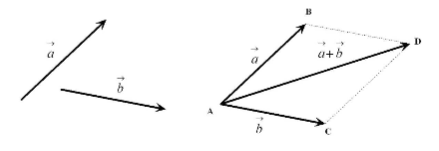
\includegraphics{sum_vec1}\\
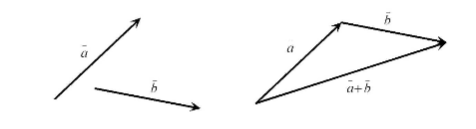
\includegraphics{sum_vec2}\\
\subsection{Произведение вектора и действительного числа}
Произведение дейсвительного числа альфа ($ \alpha \in R $) и $ \vec{a} $ называется вектор, обозначаемый $ \alpha\vec{a} $ длинна которого равна $ |\alpha||\vec{a}| $ а направление определяется следующим образом:\\
1. Если альфа больше нуля то $ \vec{a} $ и $ \alpha\vec{a} $ сонаправленны\\
2. Если альфа меньше нуля то $ \vec{a} $ и $ \alpha\vec{a} $ противоположно направленны\\
3. Если альфа равно нулю то  $ \alpha\vec{a} $ нулевой\\
Свойства:\\
1.$\forall \vec{a}\vec{t} \quad\forall \alpha \in R \quad\alpha(\vec{a}+ \vec{t}) = \alpha \vec{a} + \alpha \vec{b}$\\
2.$  \forall \vec{a} \quad\forall \alpha p\in R  \quad(\alpha + p)\vec{a} = \vec{a} \alpha + \vec{a}p$\\
3. $  1 \vec{a} = \vec{a} $\\
4. $  \forall \vec{a} \quad\forall \alpha p \in R  \quad(\alpha p)\vec{a}= \alpha p\vec{a}$\\
5. $  -\vec{a} = -1\vec{a} $\\
\begin{mdframed}[backgroundcolor=blue!20] 
       Теорема: Ненулевые $ \vec{a} $ и $ \vec{b} $ коллинеарны когда и только тогда когда существует дествительное число $ \alpha $ такое что $ \vec{a} = \alpha\vec{b} $ ($\vec{a}|\vec{b} \Leftrightarrow \exists \alpha \vec{a} = \alpha\vec{b}$).
    \end{mdframed}



\subsection{Скалярное произведение векторов}
%Переделать определение, свойства 
Пусть $ \vec{a} \quad and \quad \vec{b} $:\\
Скалярным произведением векторов называется число $ \vec{a} \vec{b} = |\vec{a}|\cdot |\vec{b}|\cos \alpha $, где альфа между ними. Обозначается \textbf{'$ \cdot $'}.

Свойства:\\
1. $ \vec{a} \cdot \vec{b} = \vec{b} \cdot \vec{a} $\\
2. $ \vec{a} \cdot \vec{a} = |\vec{a}|^2 $\\
3. $ \vec{a} \cdot \vec{b} = 0 \quad \vec{a} = 0 \quad \vec{b} = 0 \quad or \quad \alpha = \vec{a}  \vec{b} = 90^0 $ \\
4. $ \forall \alpha \in R, \quad \alpha(\vec{a}+ \vec{b}) = \alpha \vec{a} + \alpha \vec{b}$\\
5. Дистрибутивность $ \alpha(\vec{a}\vec{b}) = (\alpha \vec{a}) \vec{b}$

Проекция вектора:\\
Свойства:\\
1. $ a_p + b_p = \vec{a}' + \vec{c}' $\\
2. $ \alpha a_p = \alpha \vec{a} $\\
3. $ a \vec{b} = a_p \vec{b} $\\

\newpage
Докажем дистрибутивность скалярного произведения:\\
Два вектора проецируются на ось $ \vec{c} $
\begin{mdframed}[backgroundcolor=blue!20] 
\[
	\vec{a} + \vec{b} = (a_p + b_p)\vec{c}=(\alpha \vec{c} + \beta \vec{c})\vec{c} = (\alpha + \beta)\vec{c}\vec{c} = \alpha(\vec{c}\vec{c})+ \beta(\vec{c}\vec{c})	
\]
\end{mdframed}

\subsection{Векторное произведение}
векторным произведением векторов $ \vec{a} \quad \vec{b} $ называется вектор ($ \vec{a}*\vec{b} $), длина которого равна произведению длин векторов на синус угла между ними \[  |\vec{a}* \vec{b}|=|\vec{a}||\vec{b}| \sin \alpha \] а направление определятся по правилу буравчика,т.е если смотреть из конца вектора на плоскость векторов $ \vec{a} \quad \vec{b} $, то кратчайщий поворот от a к b должен осуществлятся против часовой стрелки, причем этот вектор перпендикулярен плоскости.\\

Свойства:\\
1. $ -\vec{a}*\vec{b} = \vec{b}*\vec{a} $\\
2. $  |\vec{a}*\vec{b}| = S_p$\\
3. $  \forall \alpha \in R \quad \alpha(\vec{a}*\vec{b})=(\alpha \vec{a}) * \vec{b}=(\alpha \vec{b}) * \vec{a}$\\
4. $  (\vec{a} + \vec{b})*\vec{c} = (\vec{a}*\vec{c} + \vec{b}*\vec{c})$\\
5. $  \vec{a} || \vec{b} \Leftrightarrow \vec{a}*\vec{b} = \vec{0} $\\
нулевой вектор коллинеанер любому другому вектору.\\

\subsection{Смешанное произведение векторов}

Смешанным произведением векторов $ \vec{a},\vec{b},\vec{c} $ называется число($ (\vec{a}*\vec{b})\cdot \vec{c}) $, $ (\vec{a},\vec{b},\vec{c}) = (\vec{a}*\vec{b})\cdot \vec{c} $\\

Векторы $  \vec{a},\vec{b},\vec{c} $ называются компланарными если они лежат в одной плоскости или на параллельных плоскостях. Если комплонарные векторы отложит от одной точки то они будут лежать на одной плоскости.\\

Свойства:\\
1. Модуль смешанного произведения векторов $  \vec{a},\vec{b},\vec{c} $ равен объему параллелепипида, построенного на векторах $  \vec{a},\vec{b},\vec{c} $. ($  |(\vec{a}*\vec{b})\cdot\vec{c}|  = V_{prlp} $)\\
2. Если один из векторов нулевой, то смешанное произведение равно нулю. \\
3. При комплонарности векторов смешанное произведение равно нулю.\\
4. $ (\vec{a}*\vec{b})\cdot\vec{c} = (\vec{c}*\vec{b})\cdot\vec{a} $\\
5. $ (\vec{a},\vec{b},\vec{c}) =  -(\vec{b},\vec{a},\vec{c}) = -(\vec{a},\vec{c},\vec{b}) = \ldots $

\subsection{Координаты вектора}

\begin{mdframed}[backgroundcolor=blue!20] 
       Теорема:\\
       пусть $ \vec{a} \quad \vec{b} $ не коллинеарные векторы, лежащие в одной плоскости, тогда всякий $ \vec{v} $, лежащий в плоскости векторов $ \vec{a} \quad \vec{b} $ единственным образом представим в виде линейной комбинации векторов $ \vec{a} \quad \vec{b} $, т.е существует действительные числа x,y, они находятся единственным образом.\\

       Теорема\\
       пусть $ \vec{a} \quad \vec{b} \quad \vec{c}    $  некомплонарные векторы. тогда всякий $ \vec{v}  $ 	 единственным образом представим в виде линейной комбинации векторов $ \vec{a} \quad \vec{b} \quad \vec{c} $\\


    \end{mdframed}

Пусть $ \vec{a} \quad \vec{b} \quad \vec{c} $ некомплонарнаые векторы пусть $ \vec{v}  $  произвольный вектор, тогда существует x,y,z такие что x =  числа называются координатами вектора в афинной системе координат образованной векторами $ \vec{a} \quad \vec{b} \quad \vec{c}    $, причем векторы абс называются базисами афинной системы координат.
\[
	 \vec{v}(x,y,z)  
\]

Аналогично рассматривается афинная система координат на плоскости образованная двумя неколлериальными векторами. Частным случаем афинной системы координат является декартова система координат.\\

Единичные ортогональные векторы:
\[
	\vec{i},\vec{j},\vec{k}   
\]
-- базис пространства\\
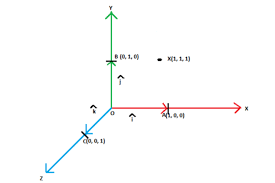
\includegraphics{orth_vec}\\

\subsection{Вычисление скалярного, векторного и смешанных произведений в прямоугольной система координат}

Скалярное
\[
	\vec{a} = (x_1,y_1,z_1) 
\]
\[
	\vec{g} = (x_2,y_2,z_2) 
\]
\[
	\vec{a}\cdot \vec{g} =   	
\]
\[
	= (x_1 \vec{i} + y_1 \vec{j} + z_1 \vec{k})\cdot(x_2 \vec{i} + y_2 \vec{j} + z_2 \vec{k})      
\]
\[
	\ldots
\]

Векторное
\[
	\vec{a} = (x_1,y_1,z_1) 
\]
\[
	\vec{g} = (x_2,y_2,z_2) 
\]
\[
	\vec{i}^2 = 0 \quad \vec{j}^2 = 0 \quad \vec{k}^2 = 0   	
\]
\[
	\vec{a}* \vec{g} =   	
\]
\[
	= (x_1 \vec{i} + y_1 \vec{j} + z_1 \vec{k})*(x_2 \vec{i} + y_2 \vec{j} + z_2 \vec{k})      
\]
\[
	\ldots
\]

\section{Система линейных уравнений. }
Рассмотрим систему линейных уравнений
\begin{align*}
	(\sum_{n=1,m=1} a_m x_n = b_1  )and(\sum_{n=1,m=1} a_m x_n = b_2)and ...and(\sum_{n=1,m=1} a_m x_n = b_n)\\	
\end{align*}
\[
	A = \begin{pmatrix}
		a_{1,1} && a_{1,1} && a_{1,m} && \ldots&&| b_1\\
		a_{2,1} && a_{2,2} && a_{2,m}&& \ldots &&| b_2\\
		&& \ldots&& \ldots&& \ldots&& \ldots\\
		a_{n,1} && a_{n,2} && a_{n,m}&& \ldots &&| b_n\\
	\end{pmatrix}
\]
-- расширенная матрица систем
\[
	AX=B
\]
-- матричная запись системы\\

Если столбец свободных членов нулевой($ b_1 = 0 \quad \ldots \quad b_n = 0 $ ), то система называется однородной, иначе неоднородной
Рассмотрим однородную систему 
\[
	A = \begin{pmatrix}
		a_{1,1} && a_{1,1} && a_{1,m} && \ldots &&| 0\\
		a_{2,1} && a_{2,2} && a_{2,m}&& \ldots &&| 0\\
		&& \ldots && \ldots && \ldots && \ldots\\
		a_{n,1} && a_{n,2} && a_{n,m}&& \ldots &&| 0\\
	\end{pmatrix}
\]
Если определитель матрицы($ det(A) $ ) не равен нулю то в силу правила Крамера система имеет единственное решение оно имеет единственное нулевое решение.

Если определитель равен нулю то система имеет бесконечно много решений, причем множество этих решений образует векторное подпространство внутри пространства $ F^m $ (последовательности из m элементов поля F)\\ 

Действительно пусть $ v_1 = v_2 $ решение системы, т.е $ Av_1 = 0 \quad Av_2 = 0 $\\
Пусть $ \alpha  \in F $\\
ТОгда \[
	A(v_1 - v_2) = 0 + 0 = 0
\]   
т.е $ v_1 + v_2  $ -- решение системы 
\newpage
\begin{mdframed}[backgroundcolor=blue!20] 
       Теорема\\
       Пусть $ Ax = 0 $ система линейных однородных уравнений, m - кол-во переменных, r - это ранг матрицы A($ m \neq r $) , тогда множество решений системы есть конечно-мерное векторное пространство размерности $ m-r $  
    \end{mdframed}
Алгоритм нахождения базиса пространства решений однородной системы\\
1) находим ранг матрицы системы с помощью элементарных преобразований, при этом преобразуем матрицу так чтобы вненулевых строках на главной диоганали элементы были ненулевые
\[
	\begin{pmatrix}
		+ && + && + && + \\
		0 && + && + && + \\
		0 && 0 && + && + \\
		0 && 0 && 0 && 0 \\
	\end{pmatrix}
\]

$ \quad \quad \quad \quad \quad \quad \quad \quad \quad  $ (трапецеевидной формы),\\
 переменные ненулеввые коэфиценты которых находятся на главной диоганали мы быдим называть базесными(главными) а остальные свободными. Если ранг матрицы находится методом окрамляющих миноров то главные элементы это те коэфиценты которых входят в матрицу наибольшего ненулевого минора\\
2) Подставляем по очереди вместо одной из свободных переменных единицу а остальные нули. РЕшаем получившиеся системы и получаем векторы $ v_1,v_2,\dots,v_{m-r} $\\
3) Записываем ответ в виде $ c_1v_1 + c_2v_2 + \ldots + c_{m-r}v_{m-r} $\\
где $ c_1 + c_2 + \ldots + c_{m-r} = const$\\

\begin{mdframed}[backgroundcolor=blue!20] 
         Теорема Кронейкера-Капели\\
         Пусть Ax = b неоднородная система линеных уравнений, тогда Ax = b имеет решения тогда и только тогда когда ранг $ A $  = рангу матрицы $ \overline{A} $. \\

         Теорема\\
         Пусть Ax= b система линейных неоднородных уравнений, m - кол-во переменных, r - ранг матрицы($ m \neq r $ ).\\
         Пусть $ v_1,v_2  $ и тогдалие - базис пространства решения однородной системы Ax=0, тогда всякое решени системы Ax=b имеет вид $ c_1v_1 + c_2v_2 + \ldots + c_{m-r}v_{m-r}  + v_{\text{частное}}$ \\
         где $ c_1 + c_2 + \ldots + c_{m-r} = const$\\
         где $ v_{\text{частное}} $ - любое известное решение Ax=b 
      \end{mdframed}
        
\newpage
Замечание:\\
векторы $ v_1,v_2  $ и тогдалие называют фундаментальной системой решений(ФСР)\\

















\newpage
\subsection*{Литература}
Задачи по линейной алгебре: матрецы определители Журавлев Е.В\\
!!!(для индивидуальных работ)Сборник типовых заданий и примеров по аналит геометрии Журавлев Е.В\\
Векторы Журавлев Е.В Мальцева Е.Ю\\
Лошкеева В.Д Мальцев Ю.М Высшая алгебра и аналит геометрия(изд алтгу 2000)\\
Курош А.Г Курс высшей алгебры\\
Фаддеев Д.К Лекции по алгебре\\
Проскуряков И.В Сборник задач по линейной алгебре\\
Задачи по высшей алгебре Фаддеев Д.К Саминцкий Д.С\\
!!Высшая математика в урпражнениях и задачах Домков П.Е Попов А.Г Кожевникова Т.Я\\
!!Погорелов А.В Аналитическая геометрия\\
Александров П.С Аналитическая геометрия\\
Геометрия. Учебник для 10 -11 классов Атанасян\\



\end{document}